\chapter{Referencial Teórico}
\label{chap:refteorico}

Nesta seção será apresentada o embasamento teórico para desenvolvimento do projeto.

%================================================================================
\section{Sistemas de Visão Computacional}
\label{sec:sistemasVisaoArtificial}

Um sistema de visão computacional é composto por etapas, sendo elas: definição do problema, aquisição da imagem, pré-processamento, segmentação, identificação do objeto e reconhecimento de padrões, como visto na Figura~\ref{fig:acoesProcImagem}.

\begin{figure}[!hbtp]
  \centering
   \caption{Ações de Aquisição e Processamento de Imagem.}
    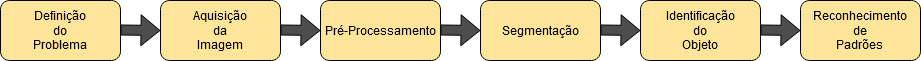
\includegraphics[width = 0.8\textwidth]{Caps/Figs/ref-teorico/acoes-procImagem.jpg}
   \label{fig:acoesProcImagem}
    \fonte{Autor}
\end{figure}

\subsection{Definição do Problema}
\label{subsec:defProblema}

Para \citeauthor{rogeralex1999} (\citeyear{rogeralex1999}), a primeira etapa do processo é a definição do problema, ou seja, qual é o objetivo que o sistema deve cumprir. Este pode ser a identificação de peças numa esteira rolante, a identificação de impressões digitais ou o reconhecimento de obstáculos na trajetória de um robô móvel. Se o sistema tiver sido bem planejado, chega-se a última etapa do processo, que é o resultado, ou seja, qual é a peça, a quem pertence a impressão digital ou qual é o obstáculo do robô.

\subsection{Aquisição da Imagem}
\label{subsec:aquisImagem}

Nesta etapa necessita-se de um dispositivo sensível a faixa do espectro eletromagnético desejado, também conhecido como câmera. Estes equipamentos que compõe o ambiente produzem em sua saída um sinal elétrico proporcional a quantidade de energia captada. Esse sinal elétrico, precisa então passar por um conversor analógico-digital para que possa ser processado pelo computador \cite{rogeralex1999}.

\subsection{Pré-processamento da Imagem}
\label{subsec:preProcImagem}

Após digitalizar e armazenar a imagem em um computador, as técnicas de pré-processamento são usadas para aprimorar a qualidade de uma imagem, corrigindo iluminação, contraste, distorções e nitidez~\cite{rudek2001visao}.

Essas operações podem ser realizadas tanto no domínio espacial quanto no domínio da frequência. O domínio espacial refere-se ao próprio plano da imagem e é caracterizado pela manipulação direta dos \textit{pixels}. As técnicas de processamento no domínio da frequência são baseadas na manipulação da Transformada de Fourier da imagem~\cite{rogeralex1999}.

\subsection{Segmentação da Imagem}
\label{subsec:segImagem}

\citeauthor{heinen2004navegaccao} (\citeyear{heinen2004navegaccao}) afirma que em processamento de imagens, segmentar consiste em identificar e extrair estruturas homogêneas presentes em uma cena, sendo a eficiência deste processo diretamente relacionada ao desempenho final da análise automática de imagens. É importante enfatizar que essa é uma etapa crítica do processo.

Esta técnica é utilizada para reduzir o esforço computacional, reduzindo as informações da imagem. Para~\citeauthor{rudek2001visao} (\citeyear{rudek2001visao}), a ideia utilizada na segmentação (\textit{thresholding}) é dividir a imagem em regiões que correspondem a unidades estruturais da cena, ou que distinguem os objetos de interesse, separando os objetos da imagem (\textit{foreground}) das informações de fundo da imagem (\textit{background}). Com esta abordagem, minimiza-se o tamanho do espaço de onde as informações são retiradas, diminuindo o esforço computacional necessário para tratar a imagem.

A dificuldade normalmente encontrada está no fato de não haver conhecimento a priori do número e tipo de estruturas presentes na imagem. Estas são identificadas a partir de características como forma, geometria, topologia, textura, cor ou brilho, sendo escolhidas aquelas que possibilitam melhor distinção~\cite{heinen2004navegaccao}.

\subsection{Identificação do Objeto}
\label{subsec:idObjeto}

Visto que os elementos de interesse da imagem foram individualizados, deve-se determinar a melhor forma de representá-los, isto é, se apenas o seu contorno já contém a informação necessária ou se todos os \textit{pixels} são necessários para a identificação do objeto. Portanto, deve-se determinar características do objeto que possam contribuir para a sua identificação.

\citeauthor{rudek2001visao} (\citeyear{rudek2001visao}) afirma que devido a uma variedade de razões, os dados de imagens usados na entrada de um sistema de visão, nem sempre são perfeitos. Os problemas que frequentemente ocorrem estão relacionados com a oclusão, onde um objeto pode estar parcialmente escondido atrás de outro objeto. 

De forma análoga, a perda de informações ou deformações, podem ser ocasionadas por ruídos na imagem devido a condições anormais de iluminação, defeitos de digitalização, e de resultados ineficientes de algoritmos de segmentação~\cite{beis1999indexing}.

\subsection{Reconhecimento de Padrões}
\label{subsec:recPadroes}

As técnicas de reconhecimento de padrões, tratam da identificação de partes da imagem que possuem semelhanças. Uma grande quantidade de ferramentas matemáticas e computacionais, tem sido desenvolvidas para permitir que objetos possam ser extraídos e agrupados em classes específicas de informações. Uma boa representação da forma do objeto, gera facilidades para que ele seja armazenado, transmitido, comparado, reconhecido ou mesmo entendido. A representação deve ser gerada de acordo com regras simples e precisas. Geralmente uma forma é descrita em termos de número de componentes, primitivas e relacionamentos entre estes componentes~\cite{rudek2001visao}.

%================================================================================
\section{Métodos de Visão Computacional}
\label{sec:metodos-visaoComputacional}

Diversas técnicas para a segmentação de imagens em sistemas de visão computacional foram desenvolvidas de acordo com o objetivo do RMA. Algumas utilizam duas câmeras e outros apenas uma, e estas podem estar dispostas fixas ao robô ou no ambiente. Para \citeauthor{araujo2008reconhecimento} (\citeyear{araujo2008reconhecimento}), os métodos de visão computacional se agrupam em três formas de reconhecimento: baseado em cores, baseado em forma, e baseado em cores e forma.

\begin{itemize}
    \item \textbf{Sistema baseado em cores:} A câmera registra a cor da luz refletida pela superfície, que depende tanto da cor da superfície como da cor da iluminação. Entretanto, a cor da iluminação pode variar bastante, como, por exemplo, é azul para iluminação fluorescente, laranja para incandescentes, e vermelha ao pôr do sol~\cite{konzen2007problema}.
    
    \item \textbf{Sistema baseado em forma:} A câmera registra determinadas formas geométricas, que são utilizadas para detectar unicamente cada objeto~\cite{garcia2007arcaboucco}.
    
    \item \textbf{Sistema baseado em cores e forma:} Sistema híbrido que faz a identificação através do reconhecimento baseado em forma e a individualização baseada em cores~\cite{martins2007towards}.
\end{itemize}


\citeauthor{andrade2006sistema} (\citeyear{andrade2006sistema}), propõe um sistema onde duas câmeras são dispostas no ambiente e executam uma triangulação. Ainda cita que, \citeauthor{souza2003desenvolvimento} (\citeyear{souza2003desenvolvimento}) propõe um sistema baseado na limiarização das cores dos componentes da imagem através das proporções de seus componentes vermelho, verde e azul, e; \citeauthor{penharbel2004filtro} (\citeyear{penharbel2004filtro}), utilizam os componentes vermelho, verde e azul dos \textit{pixels} para obter o tom, saturação, e a intensidade das cores, a fim de efetuar a limiarização sobre este último espaço de valores.

\subsection{Triangulação com Câmeras no Ambiente}
\label{subsec:triangulacao}

Uma das propriedades mais relevantes deste sistema é o fato de que ele opera extraindo imagens a partir de duas câmeras. Uma delas é posicionada perpendicularmente ao plano de operação do robô e outra de forma inclinada. O interesse em uma segunda câmera com posição inclinada é, além de tornar a análise da cena mais robusta, tornar possível a detecção de obstáculos finos e alongados verticalmente, o que poderia ser tratado como ruído e passar despercebido no sistema de visão \cite{andrade2006sistema}.

A princípio, a imagem capturada pela câmera é pré-processada pelo sistema, visando eliminar seu fundo. Para isso, pode-se utilizar técnicas de limiarização, que é o processo de segmentação de imagens que se baseia na diferença dos níveis de cinza que compõe diferentes objetos de uma imagem.

\citeauthor{andrade2006sistema} (\citeyear{andrade2006sistema}) explicam que, no pré-processamento das imagens seguintes, a cor a ser tida como padrão durante a rotulação dos \textit{pixels} é definida como a média temporal de todas as cores obtidas até então. Essa medida evita que mudanças bruscas no ambiente afetem o funcionamento do sistema. A segmentação do robô também utiliza a limiarização, e são segmentados os \textit{pixels} cuja distância no espaço tricromático a cor de frente ou a de fundo do robô (definidas pelo usuário na inicialização do sistema) é inferior a um limiar. A área do robô é calculada pelo somatório dos seus \textit{pixels}, sua posição é definida como sendo as coordenadas de seu centro de área, e sua orientação é definida como o ângulo formado pela semi-reta que tem como origem o centro de área da região do fundo do robô e passa pelo centro de área da região de sua frente. O processo utilizado na verificação de obstáculos é baseado em um sonar visual, onde são utilizados 18 feixes que saem do centro de área do robô em diferentes ângulos e vão percorrendo a imagem \textit{pixel} a \textit{pixel}. A varredura de cada feixe termina quando ele encontra um obstáculo ou quando atinge um dos limites da imagem. As coordenadas dos pontos de parada de cada feixe são guardadas em um vetor, que é passado para o sistema de controle juntamente com as características do robô.

O sistema desenvolvido por \citeauthor{andrade2006sistema} (\citeyear{andrade2006sistema}), pode ser visto na Figura~\ref{fig:triangulacao}.

\begin{figure}[!hbtp]
  \centering
   \caption{Processo de Extração de Características.}
    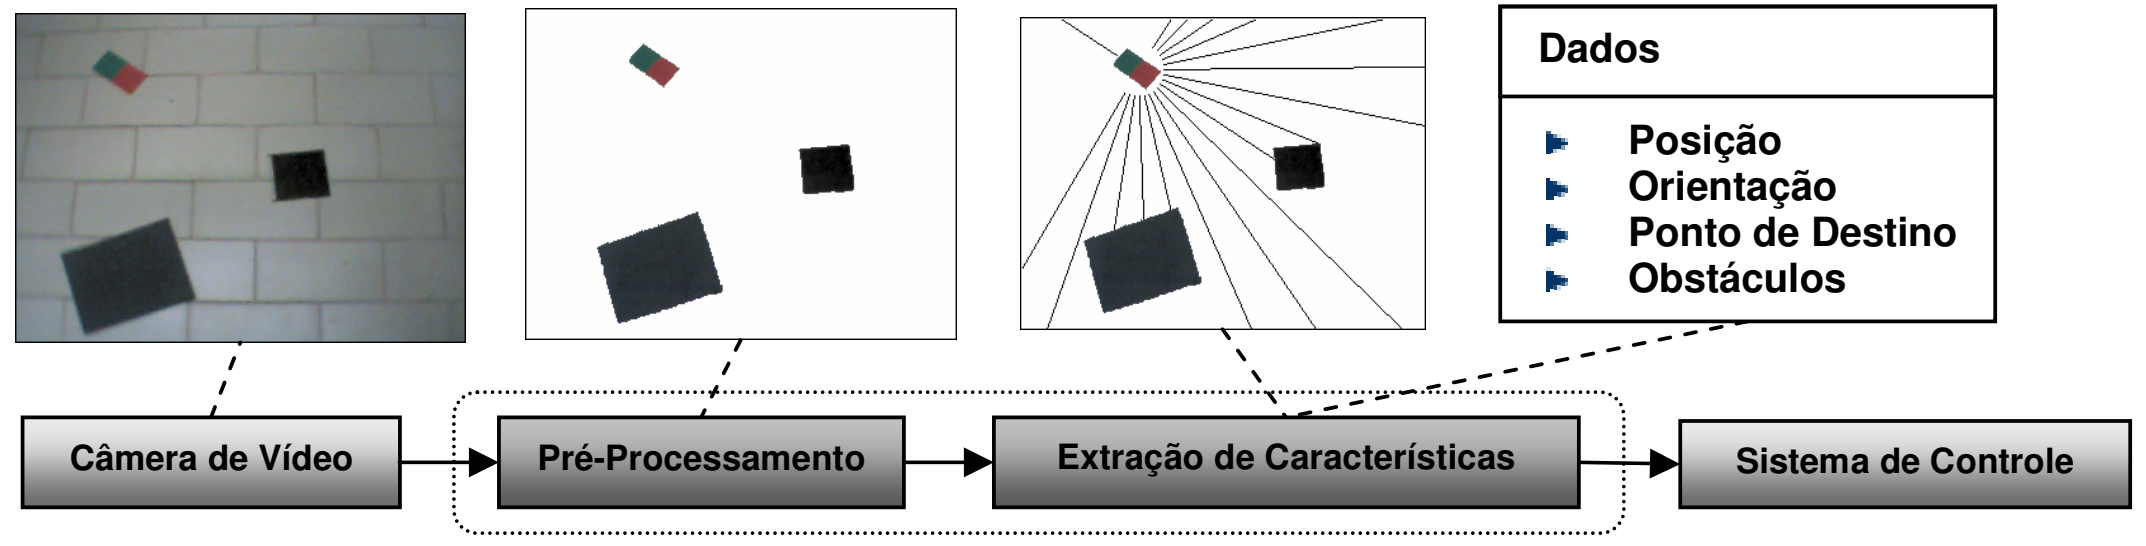
\includegraphics[width = 0.8\textwidth]{Caps/Figs/ref-teorico/triangulacao.png}
   \label{fig:triangulacao}
    \fonte{\cite{andrade2006sistema}}
\end{figure}


\subsection{RGB}
\label{subsec:rgb}
\nomenclature{RGB}{\textit{Red, Green e Blue}}
\nomenclature{CIE}{Comissão Internacional de Iluminação}

Objetos que emitem luz visível são percebidos em função da soma das cores espectrais emitidas. Tal processo de formação é denominado aditivo. O processo aditivo pode ser interpretado como uma combinação variável em proporção de componentes monocromáticas nas faixas espectrais associadas às sensações de cor verde, vermelho e azul, as quais são responsáveis pela formação de todas as demais sensações de cores registradas pelo olho humano. Assim, as cores verde, vermelho e azul são ditas cores primárias. Este processo de geração suscitou a concepção de um modelo cromático denominado RGB (\textit{Red, Green e Blue}), para o qual a Comissão Internacional de Iluminação (CIE) estabeleceu as faixas de comprimento de onda das cores primárias~\cite{de2006introduccao}, visto na Figura~\ref{fig:modeloRGB}.

\begin{figure}[!hbtp]
  \centering
   \caption{Modelo RGB.}
    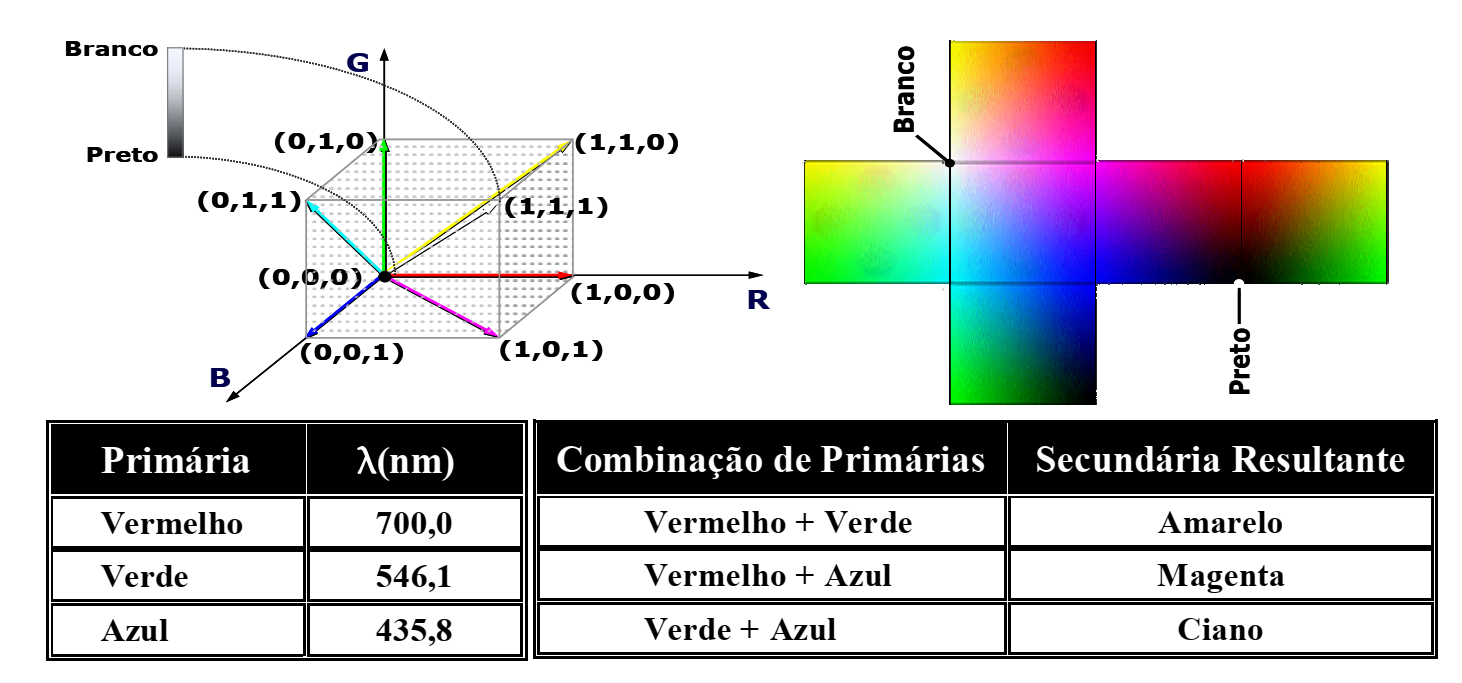
\includegraphics[width = 0.8\textwidth]{Caps/Figs/ref-teorico/modelo-RGB.png}
   \label{fig:modeloRGB}
    \fonte{\cite{de2006introduccao}}
\end{figure}

\subsection{HSV}
\label{subsec:hsv}
\nomenclature{HSV}{\textit{Hue, Saturation} e \textit{Value}}

O espaço de cores HSV (\textit{Hue, Saturation} e \textit{Value}) particiona uma cor em matiz, saturação e intensidade, sendo a matiz a cor propriamente dita, a saturação identifica o quão forte é a cor, e a intensidade identifica a luminância da cor. O espaço de cores HSV forma um cone, com H variando de 0 a 360 graus e S e I variando de 0 a 100 por cento~\cite{penharbel2004filtro}. A Figura~\ref{fig:modeloHSV} permite visualizar esse espaço.

\begin{figure}[!hbtp]
  \centering
   \caption{Modelo HSV.}
    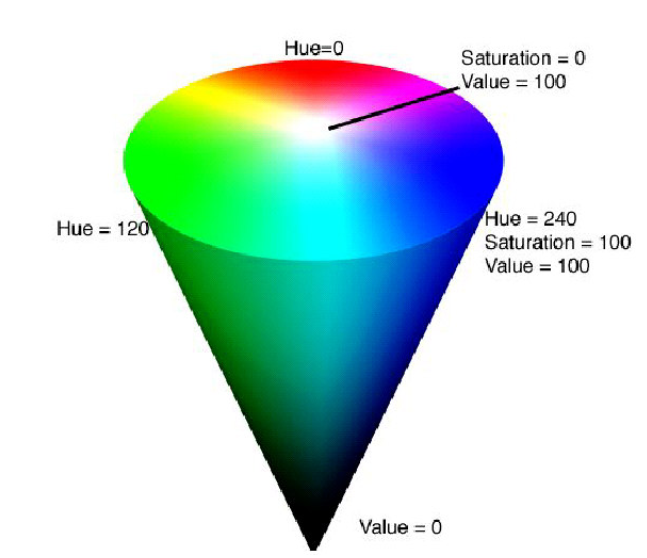
\includegraphics[width = 0.8\textwidth]{Caps/Figs/ref-teorico/modelo-HSV.png}
   \label{fig:modeloHSV}
    \fonte{\cite{penharbel2004filtro}}
\end{figure}

\citeauthor{penharbel2004filtro} (\citeyear{penharbel2004filtro}), descreve que esse espaço de cores é propício para filtro que precisa separar cores independente da luminosidade. O grande problema de usar o espaço de cores HSV se dá pela necessidade de transformação de cada \textit{pixel} da imagem, originalmente em RGB proveniente da câmera de vídeo, para o formato HSV, o que gasta tempo de processamento e que pode tornar o filtro computacionalmente ineficiente.

\subsection{Histogramas}
\label{subsec:histogramas}

Os histogramas são definidos por~\citeauthor{marengoni2009tutorial} (\citeyear{marengoni2009tutorial}) como ferramentas de processamento de imagens que possuem grande aplicação prática. Os histogramas são determinados a partir de valores de intensidade dos \textit{pixels}. Entre as principais aplicações dos histogramas estão a melhora da definição de uma imagem, a compressão de imagens, a segmentação de imagens ou ainda a descrição de uma imagem.

Para melhor entendimento, \citeauthor{hoshiro2008processamento} (\citeyear{hoshiro2008processamento}) define o histograma como semelhante a um gráfico de frequências, onde cada pilha representa uma cor identificada em um \textit{pixel} de um uma imagem. É muito utilizado para cálculos estatísticos em imagens e recuperação de imagens.

O histograma de uma imagem I, cujos valores de intensidade estejam entre 0 e G é definido pela Equação~\ref{eq:defHistograma}:
\begin{equation}
\label{eq:defHistograma}
    h(I_k) = n_k
\end{equation}

onde $I_k$ é um valor de intensidade $k$, $(0\leq k\leq G)$ da imagem I e $n_k$ é o número de \textit{pixels} na imagem I que possuem a intensidade k. É possível normalizar um histograma, representando os valores de em termos de porcentagem, como mostrado na Equação~\ref{eq:normHistograma}:
\begin{equation}
\label{eq:normHistograma}
    p(I_k) = \frac{h(I_k)}{n} = \frac{n_k}{n}
\end{equation}

onde $n$ é o número de \textit{pixels} na imagem. A Figura~\ref{fig:modeloHistrograma} mostra como um histograma é determinado.

\begin{figure}[!hbtp]
  \centering
   \caption{À esquerda uma imagem I, ao centro o histograma da imagem em valores (h(I)) e em porcentagem (p(I)), à direita uma representação do histograma de forma gráfica.}
    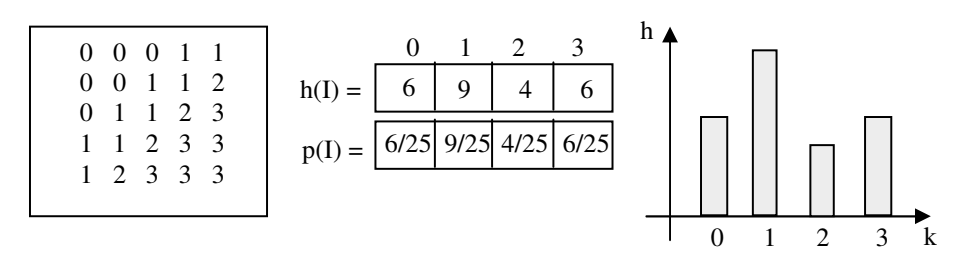
\includegraphics[width = 0.8\textwidth]{Caps/Figs/ref-teorico/histogram.png}
   \label{fig:modeloHistrograma}
    \fonte{\cite{marengoni2009tutorial}}
\end{figure}


%================================================================================
\section{OpenCV}
\label{sec:opencv}
\nomenclature{OpenCV}{\textit{Open Source Computer Vision Library}}
\nomenclature{GUI}{Interface Gráfica do Usuário}


OpenCV (\textit{Open Source Computer Vision Library}) é uma biblioteca multiplataforma de código aberto, originalmente desenvolvida pela Intel, para o desenvolvimento de aplicativos na área de visão computacional. Essa possui módulos de processamento de imagens, estrutura de dados, álgebra linear e GUI (Interface Gráfica do Usuário) básica, além de mais de 350 algoritmos de visão computacional, como: filtros de imagem, calibração de câmera, reconhecimento de objetos, análise estrutural e outros.

\citeauthor{bradski2008learning} (\citeyear{bradski2008learning}) afirma que a OpenCV foi desenvolvida com o intuito de eficiência computacional e com um grande foco em aplicações de tempo real. Esta é escrita em C/C++, porém hoje contém interfaces de desenvolvimento para diversas linguagens, tais como Python, Ruby, Matlab e outras.

\citeauthor{baggio2015opencv} (\citeyear{baggio2015opencv}) complementa que desde seu lançamento suas funcionalidades vem sendo desenvolvidas pela comunidade científica, tornando esta biblioteca uma ferramenta poderosa no campo da visão computacional.

\subsection{Rastreamento de objetos}
\label{subsec:rastreamentoObjtos}

O processo de rastreamento é um processo de reconhecer um padrão em uma sequência de imagens. O rastreamento poderia ser feito desta forma, porém, a busca em cada imagem de uma sequência sem o uso de qualquer conhecimento específico é relativamente lenta. Os processos de rastreamento atrelam um conhecimento sobre o movimento do objeto que está sendo rastreado para minimizar a busca entre as imagens em uma sequência. Os processos de rastreamento podem ser aplicados em diversas áreas, indo de sistemas de segurança/vigilância até o uso em sistemas de interface humano-computador. Existem métodos para se prever a posição do objeto \textit{frame} a \textit{frame}, indo de filtros de Kalman, até processos com filtros de partículas. No OpenCV as técnicas de rastreamento incluem dois componentes principais: identificação de objetos e modelagem da trajetória. Existem algumas funções que são utilizadas para o rastreamento, baseadas nos algoritmos de "\textit{Meanshift}" e "\textit{Camshift}"~\cite{marengoni2009tutorial}.

\subsubsection{\textit{Meanshift}}
\label{subsubsec:meanshift}

O algoritmo \textit{Meanshift} (deslocamento médio) é um método robusto de análise de espaço para localizar os máximos de uma função de densidade de um conjunto de dados. Este é um processo fácil para distribuições contínuas, porém para conjuntos de dados discretos esse problema é um pouco menos trivial. O termo robusto é usado aqui com seu sentido estatístico, isto é, o algoritmo ignora pontos de dados que estão longe dos picos. Ele faz isso processando apenas pontos em uma janela local de dados e, em seguida, movendo essa janela~\cite{bradski2008learning}.

Ele executa da seguinte maneira:
\begin{enumerate}
    \item Escolhe uma janela de procura:
    \begin{itemize}
        \item Localização inicial;
        \item Tipo da distribuição (uniforme, polinomial, exponencial ou Gaussiana);
        \item Formato da janela (simétrica, arredondada ou retangular);
        \item Tamanho da janela;
    \end{itemize}
    \item Encontra o maior valor na janela (possivelmente ponderado).
    \item Centraliza a janela no valor encontrado no passo 2.
    \item Retorna para o passo 2 até a janela parar de se mover (sempre irá parar de se mover)~\footnote{As iterações são tipicamente restritas a algum número máximo ou a alguma mudança no deslocamento do centro entre as iterações; no entanto, elas certamente convergirão eventualmente~\cite{bradski2008learning}.}.
\end{enumerate}

A Figura~\ref{fig:meanshift} demonstra o algoritmo \textit{Meanshift} em ação. Uma janela inicial é definida em um \textit{array} bidimensional de pontos de dados e é centralizada sucessivamente sobre o pico local da sua distribuição de dados até a convergência.

\begin{figure}[!hbtp]
  \centering
   \caption{\textit{Meanshift} em ação.}
    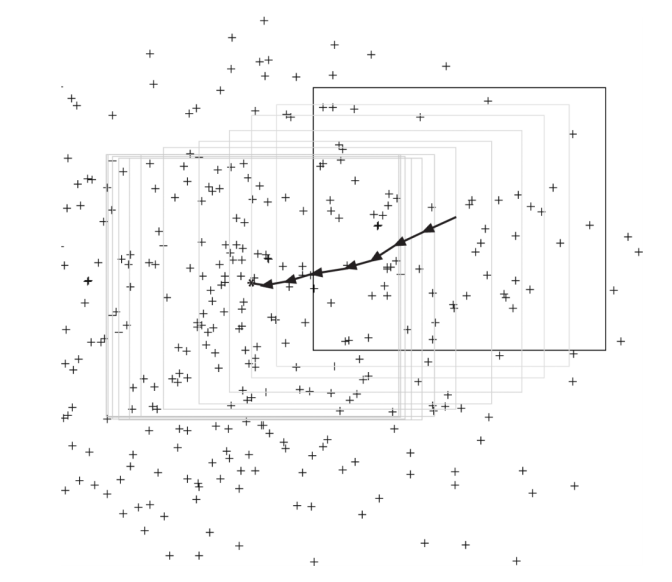
\includegraphics[width = 0.8\textwidth]{Caps/Figs/ref-teorico/meanshift.PNG}
   \label{fig:meanshift}
    \fonte{\cite{bradski2008learning}}
\end{figure}

Uma das áreas de aplicação deste algoritmo, em visão computacional, é o \textit{tracking} de objetos coloridos, onde utiliza distribuições de probabilidade para seguir objetos em \textit{frames} consecutivos. Para distribuições de probabilidade alteradas dinamicamente, que representam objetos em movimento na sequência de \textit{frames}, o algoritmo \textit{Meanshift} tem de ser modificado para se adaptar dinamicamente às alterações de tamanho e posição do objeto, nas distribuições de probabilidade~\cite{peixoto2012deteccao}. O algoritmo que consegue desempenhar tal função é chamado \textit{Camshift}, e este será abordado na Seção~\ref{subsubsec:camshift}.

\subsubsection{\textit{Camshift}}
\label{subsubsec:camshift}

O \textit{Camshift} é um algoritmo robusto, baseado no algoritmo \textit{Meanshift} (Seção~\ref{subsubsec:meanshift}). Para a utilização deste algoritmo é necessário o cálculo da função densidade de probabilidade. Esta pode ser determinada utilizando qualquer método que associe o valor de um \textit{pixel} com a probabilidade deste \textit{pixel} pertencer ao objeto alvo. Um método comum é o histograma projeção de fundo (\textit{Histogram Back-Projection}). Esta técnica recorre a comparação de histogramas, ou seja, à relação entre o histograma do objeto selecionado (janela inicial) e o histograma do \textit{frame} alvo. Desta forma, pretende-se aumentar a diferença entre o \textit{background} e o objeto, levando a uma localização mais fiel deste. O histograma projeção de fundo utiliza o canal matiz (\textit{hue}) no espaço de cor HSV, no entanto qualquer histograma multidimensional a partir de qualquer espaço de cor pode ser utilizado~\cite{peixoto2012deteccao}.

Para viabilizar o \textit{tracking} com o \textit{Camshift} é ainda necessário que o tamanho da janela se adapte ao alvo que está a ser seguido. Uma vez que o tamanho ideal da janela varia com a distância do objeto em relação a câmera. Esta adaptação é feita com base no momento de ordem zero, que pode ser interpretado como a "área" da distribuição encontrada sob a janela de pesquisa. Desta forma, o comprimento e a altura da janela são determinados em função deste momento, que consiste na soma das probabilidades de todos os \textit{pixels} na região de interesse. Como produto deste método resultam não só as coordenadas do \textit{pixel} centroide do alvo, correspondente à localização do \textit{Meanshift}, mas também a informação respeitante à área da janela ~\cite{peixoto2012deteccao}.

O algoritmo \textit{Camshift} é definido pela~\citeauthor{intel2001corporation} (\citeyear{intel2001corporation}), como:

\begin{enumerate}
    \item Defina a região de cálculo da distribuição de probabilidade para a imagem inteira.
    \item Escolha a localização inicial da janela de busca do \textit{Meanshift}.
    \item Calcule a distribuição de probabilidade de cor na região centrada na localização da janela de busca em uma região de interesse um pouco maior que o tamanho da janela de busca do \textit{Meanshift}.
    \item Faça a iteração do algoritmo \textit{Meanshift} para achar o centro da imagem de probabilidade e o momento de ordem zero.
    \item Para o próximo \textit{frame}, centralize a janela de busca na localização encontrada no passo 4 e redimensione a janela em função do momento de ordem zero. Retorne ao passo 3.
\end{enumerate}

Para \citeauthor{peixoto2012deteccao} (\citeyear{peixoto2012deteccao}), o passo inicial é estabelecer a área de interesse, para a qual é calculado o histograma que será usado como referência. A seguir centra-se a janela do \textit{Meanshift} no objeto que se pretende seguir e determina-se a distribuição de probabilidades desta região. A partir daqui o \textit{Meanshift} itera, até não haver alteração na posição, ou a alteração ser inferior a um valor previamente definido. Neste ponto estabelece a nova janela de procura e torna-se a repetir todo o processo enquanto se pretende fazer \textit{tracking} deste objeto. Um fluxograma para melhor visualização é representado pela Figura~\ref{fig:camshift}.

\begin{figure}[!hbtp]
  \centering
   \caption{Fluxograma do \textit{Camshift}.}
    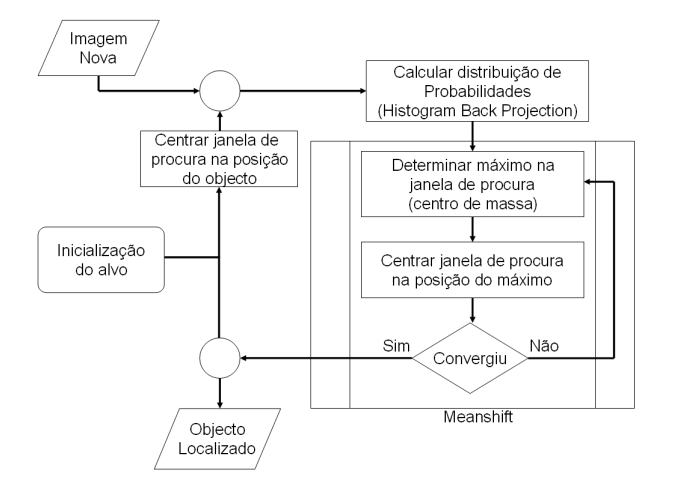
\includegraphics[width = 0.8\textwidth]{Caps/Figs/ref-teorico/camshift.png}
   \label{fig:camshift}
    \fonte{\cite{peixoto2012deteccao}}
\end{figure}

\subsubsection{Viola-Jones}
\label{subsubsec:violaJones}
\nomenclature{XML}{\textit{eXtensible Markup Language}}

A técnica proposta por Viola e Jones~\cite{viola2001rapid} permite efetuar a detecção de qualquer tipo de objeto (neste caso faces humanas) de forma genérica e em tempo real com uma taxa de sucesso bastante elevada. A abordagem proposta baseia-se em algoritmos de aprendizagem automática (\textit{machine learning}), aplicados de forma a identificar objetos, e capazes de processar imagens com muita rapidez~\cite{peixoto2012deteccao}.

Nessa técnica são utilizadas as características \textit{Haar}, as quais podem ser vistas na Figura~\ref{fig:haarfeatures}. Estas características são padrões retangulares que contém partes claras de peso positivo e partes escuras de peso negativo. Ele identifica características de bordas, linhas e centros das imagens para formar um classificador. Posteriormente foi estendido por \citeauthor{lienhart2002extended} (\citeyear{lienhart2002extended}) para usar os recursos diagonais. 

\begin{figure}[!hbtp]
  \centering
   \caption{Protótipos de características \textit{Haar}.}
    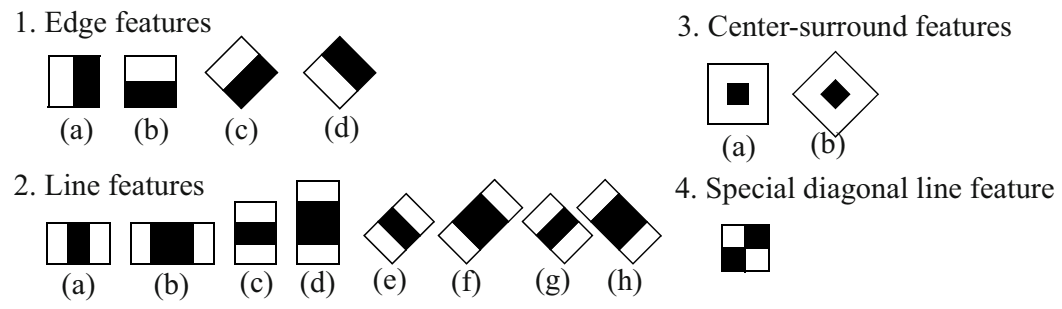
\includegraphics[width = 0.8\textwidth]{Caps/Figs/ref-teorico/haar-features.png}
   \label{fig:haarfeatures}
    \fonte{\cite{lienhart2003empirical}}
\end{figure}

A maior motivação para o uso de características de um objeto em detrimento de todos os seus \textit{pixels} é que a velocidade de análise de uma imagem baseada no conjunto de suas principais características é muito maior. Isto porque o número de características é substancialmente inferior ao número total de \textit{pixels} de um objeto~\cite{peixoto2012deteccao}.

\citeauthor{viola2001rapid} (\citeyear{viola2001rapid}) propõe três tipos de características e seus valores, sendo elas:
\begin{itemize}
    \item O valor de uma característica de dois retângulos é a diferença entra a soma dos \textit{pixels} de duas regiões retangulares iguais e adjacentes verticalmente ou horizontalmente;
    \item O valor de uma característica de três retângulos é a soma dos dois retângulos exteriores subtraída da soma do retângulo central;
    \item O valor de uma características de quatro retângulos é a diferença entre os pares diagonais.
\end{itemize}

Para simplificar o entendimento, a característica é determinada pela subtração do valor da soma de \textit{pixels} brancos com o valor da soma dos \textit{pixels} pretos. Se a características estiver acima de um limiar, dado no aprendizado do algoritmo, ela é definida como presente.

Funções de classificação tem como objetivo a classificação de objeto a partir do conjunto das duas principais características. Para encontrar essas características podem ser utilizados vários tipo de algoritmo de aprendizagem~\cite{peixoto2012deteccao}.

A fim de se obter um bom aprendizado de máquina, \citeauthor{viola2001rapid} (\citeyear{viola2001rapid}) utiliza um método variante do \textit{AdaBoost}~\cite{freund1999short}, que restringe cada classificador fraco para depender de apenas uma característica. Como resultado, cada estágio do processo de \textit{boosting} seleciona um novo classificador fraco, isto pode ser visto como um processo de seleção de características. Em seguida, ele combina classificadores fracos para formar um classificador forte. Portanto, o classificador forte é uma combinação ponderada de classificadores fracos.

Por último, estes classificadores fortes são agregados e formam uma cascata (por isso o algoritmo é conhecido também como \textit{Haar-Cascade}) de decisões, visto na Figura~\ref{fig:deteccaoCascade}. Se todas as características passarem por esse "filtro" é gerado um documento XML (\textit{eXtensible Markup Language}) para armazená-las (para melhorar o aprendizado do algoritmo), e a face é detectada.

\begin{figure}[!hbtp]
  \centering
   \caption{Detecção em cascata (\textit{Haar-Cascade}).}
    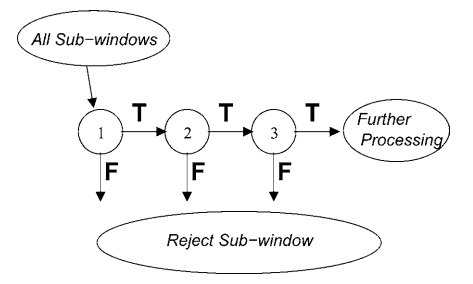
\includegraphics[width = 0.8\textwidth]{Caps/Figs/ref-teorico/detecCascade.png}
   \label{fig:deteccaoCascade}
    \fonte{\cite{viola2001rapid}}
\end{figure}

\subsubsection{YOLO}
\label{subsubsec:yolo}
\nomenclature{YOLO}{\textit{You Only Look Once}}
\nomenclature{CPU}{\textit{Central Processing Unit}}
\nomenclature{GPU}{\textit{Graphics Processing Unit}}

Os humanos olham para uma imagem e sabem instantaneamente quais objetos estão na imagem, onde estão e como interagem. O sistema visual humano é rápido e preciso, permitindo-nos realizar tarefas complexas como dirigir com pouco pensamento consciente. Algoritmos rápidos e precisos para detecção de objetos permitiriam que os computadores dirigissem carros sem sensores especializados, habilitaria dispositivos auxiliares para transmitir em tempo real informações da cena para usuários humanos, e desbloquear o potencial para uso geral em sistemas robóticos responsivos~\cite{Redmon_2016_CVPR}. Com essa percepção surge o conceito do algoritmo YOLO (\textit{You Only Look Once}).

YOLO é um método de detecção de objetos de passada única (\textit{single pass}) que utiliza uma rede neural convolucional como extrator de características (\textit{features}). Diferente de outros algoritmos de detecção de objetos (como o Viola-Jones, Seção~\ref{subsubsec:violaJones}), ele apenas precisar olhar pela imagem uma única vez para enviar para a rede neural. Por isso ele recebe esse nome (You Only Look Once – “Você só olha uma vez”)~\cite{alvesGabriel2020}. Antes do YOLO, sistemas de detecção de objetos faziam a detecção por meio da divisão da imagem em várias partes e depois em cada pedaço da imagem se executava um classificador. É necessário executar o mesmo classificador dezenas ou milhares de vezes sobre a mesma imagem.

\begin{figure}[!hbtp]
  \centering
   \caption{Sistema de detecção YOLO.}
    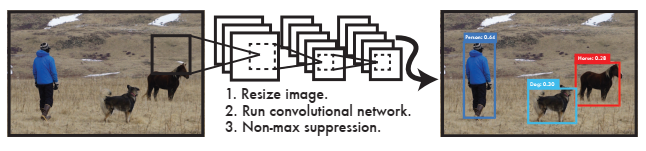
\includegraphics[width = 0.8\textwidth]{Caps/Figs/ref-teorico/YOLO-detection.png}
   \label{fig:YOLOcdetectionSystem}
    \fonte{\cite{Redmon_2016_CVPR}}
\end{figure}

O YOLO utiliza uma rede neural profunda, cuja arquitetura é chamada de \textit{Darknet} (que é o mesmo nome do \textit{framework} utilizado para implementar). Esta rede neural utiliza as características da imagem inteira para detectar múltiplas caixas, cada uma contendo um objeto. É escrita na linguagem C, e suporta CPU (\textit{Central Processing Unit}) e GPU (\textit{Graphics Processing Unit}). Foi desenvolvida inicialmente por Joseph Redmon~\cite{Redmon_2016_CVPR}, criador do YOLO.

Este sistema de visão computacional é de uso geral, proporcionando um grande avanço em áreas como medicina e robótica. Um estudo feito por \citeauthor{al2018simultaneous} (\citeyear{al2018simultaneous}), propõe o uso desta ferramenta de visão computacional para a detecção de câncer de mama, o qual é ilustrado na Figura~\ref{fig:YOLOcancerMAMA}.

\begin{figure}[!hbtp]
  \centering
   \caption{Detecção de câncer de mama pela ferramenta YOLO.}
    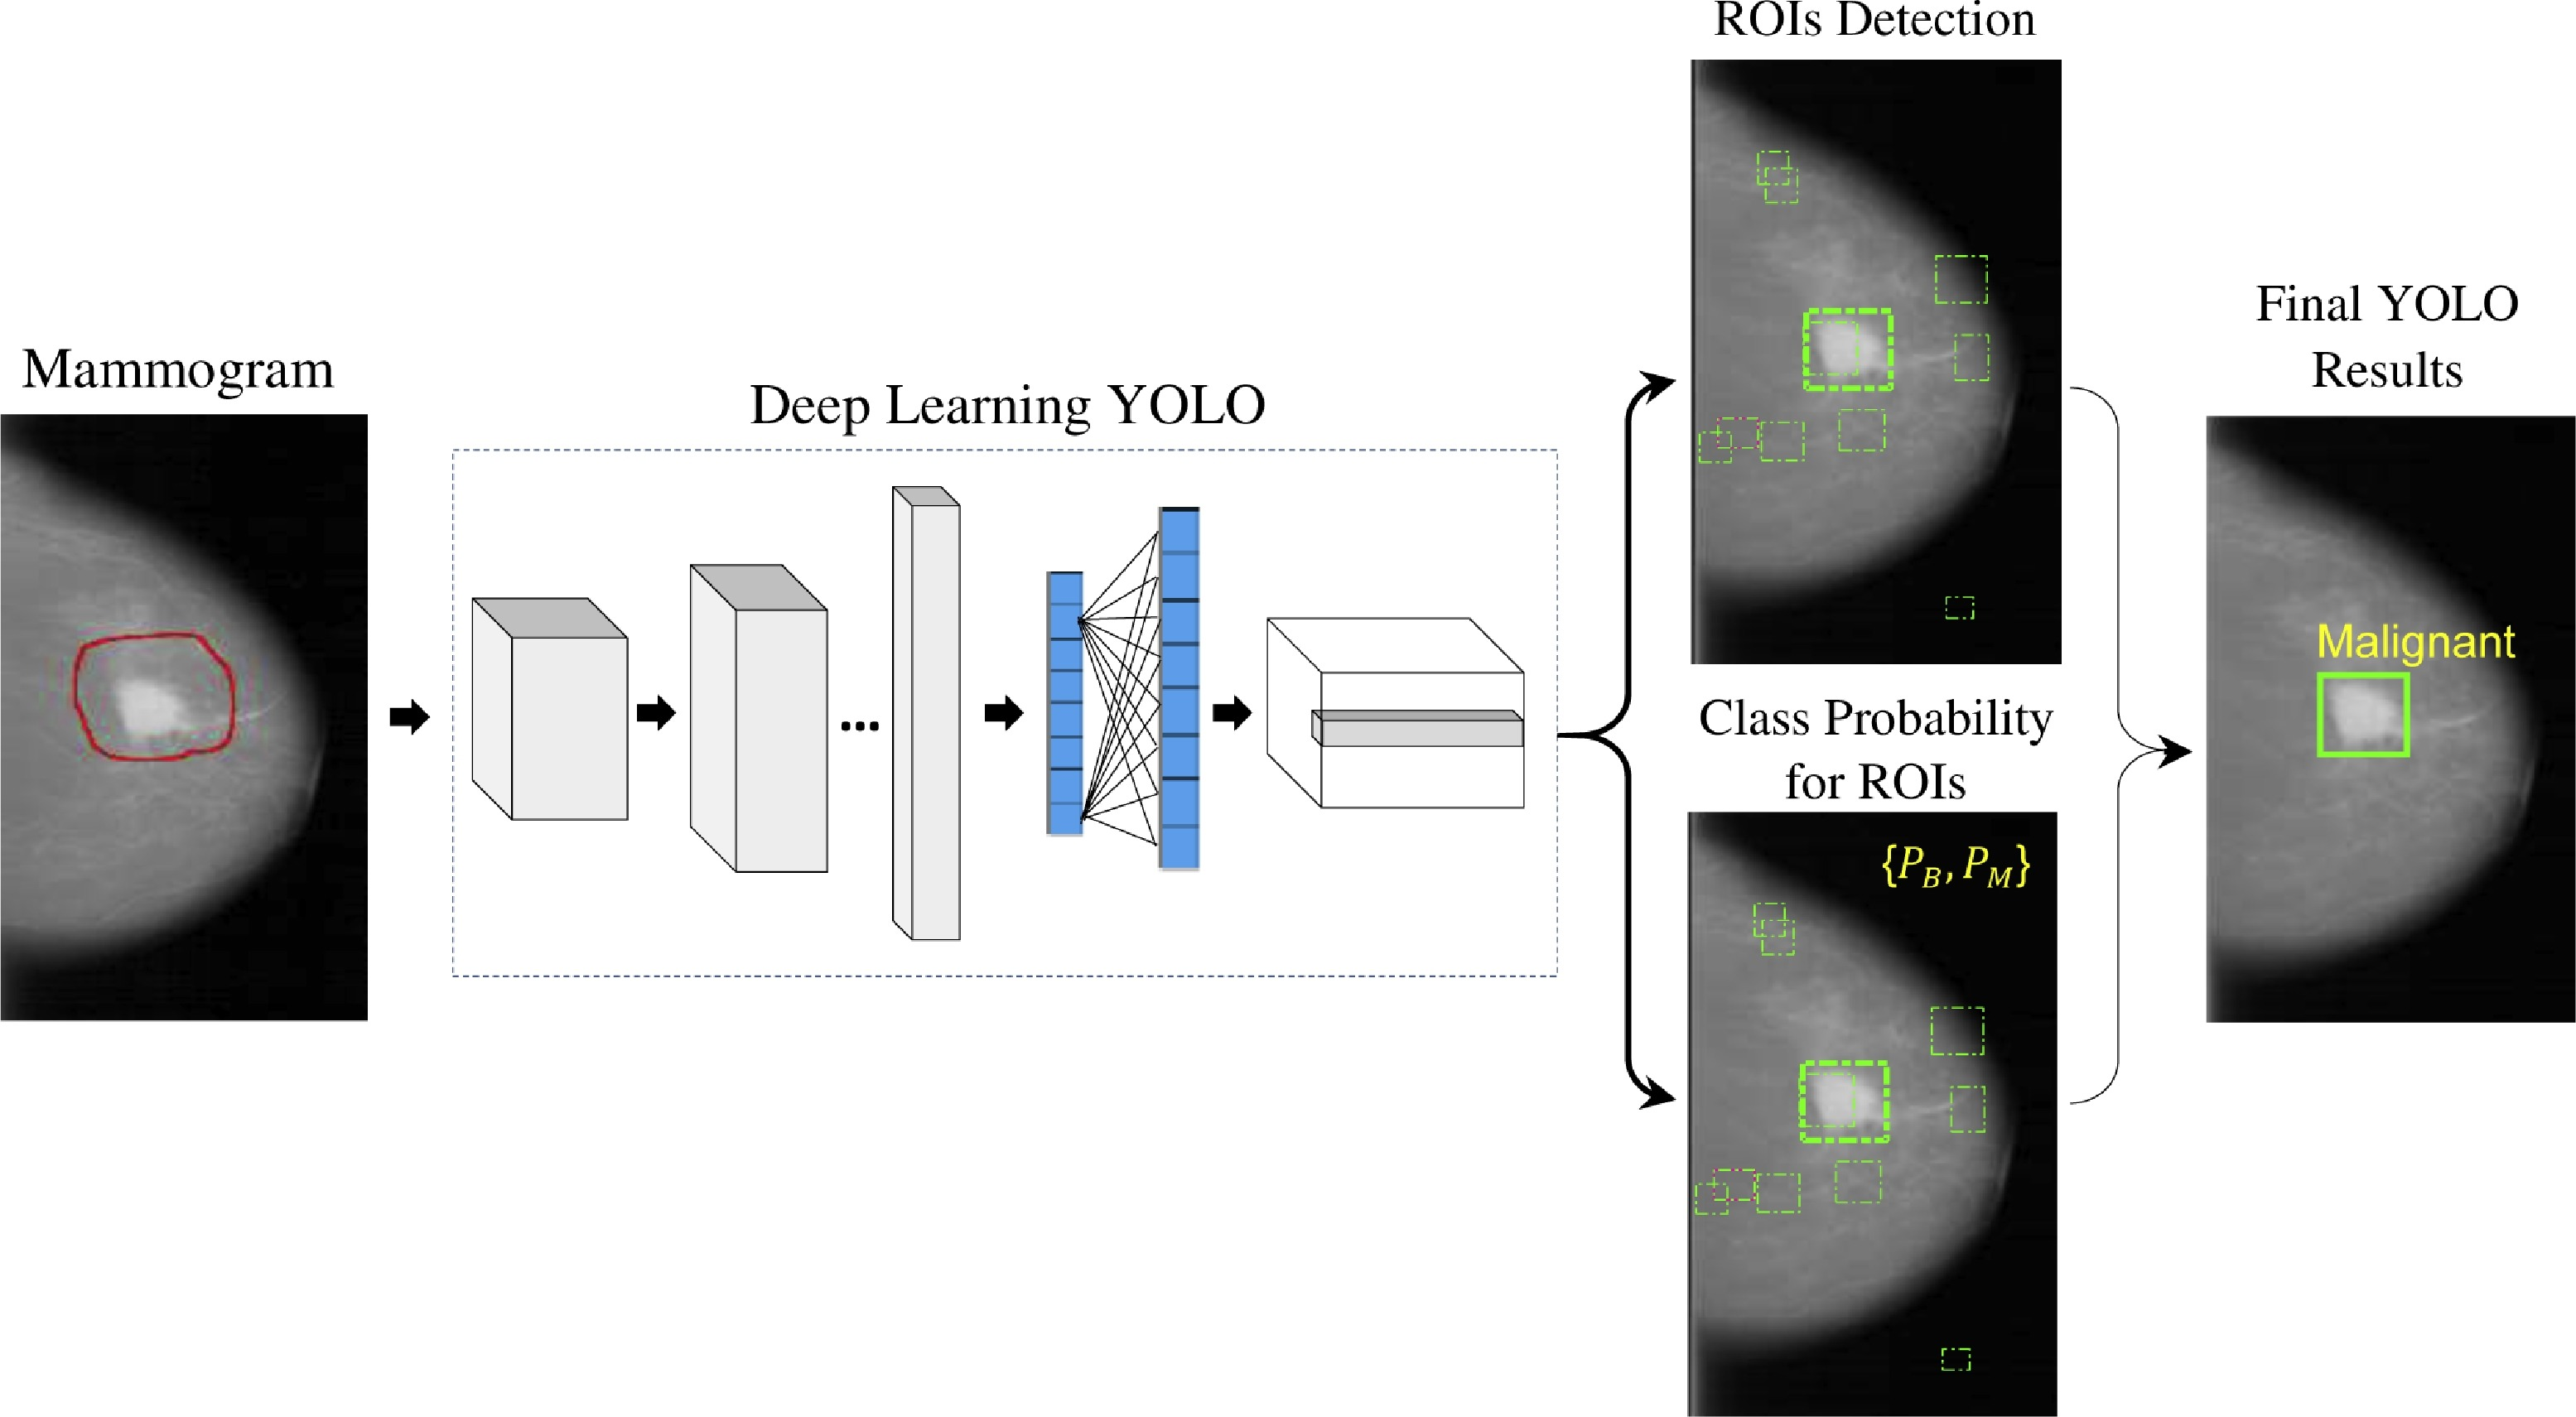
\includegraphics[width = 0.8\textwidth]{Caps/Figs/ref-teorico/YOLO-breastCancer.jpg}
   \label{fig:YOLOcancerMAMA}
    \fonte{\cite{al2018simultaneous}}
\end{figure}

Neste trabalho, propõe-se o uso do YOLO para implementar visão computacional em um RMA. Seu funcionamento é discutido na Seção~\ref{sec:matmetYOLO}.

%================================================================================
\subsection{Redes Neurais Artificiais}
\label{sec:redesneuraisArtificiais}
\nomenclature{ANN}{\textit{Artificial Neural Network}}

Redes neurais artificiais, do inglês \textit{Artificial Neural Network} (ANN), são técnicas computacionais que apresentam um modelo matemático inspirado na estrutura neural de organismos inteligentes e que adquirem conhecimento através da experiência. Uma grande rede neural artificial pode ter centenas ou milhares de unidades de processamento; já o cérebro de um mamífero pode ter muitos bilhões de neurônios. Uma rede neural artificial é composta por várias unidades de processamento, cujo funcionamento é simples. Essas unidades geralmente são conectadas por canais de comunicação que estão associados a determinado peso. As unidades fazem operações apenas sobre seus dados locais, que são entradas recebidas pelas suas conexões. O comportamento inteligente vem das interações entre as unidades de processamento da rede~\cite{andreCarvalhoRNA}.

McCulloch-Pitts~\cite{830886} propõe um modelo de operação de uma unidade de processamento, que é resumido da seguinte maneira:
\begin{itemize}
    \item Sinais são apresentados a entrada;
    \item Cada sinal é multiplicado por um número, ou peso, que indica a sua influência na saída da unidade;
    \item É feita a soma ponderada dos sinais que produz um nível de atividade;
    \item Se este nível de atividade exceder um certo limite a unidade produz uma determinada resposta de saída.
\end{itemize}

Assim como acontece no sistema nervoso, o sinal resultante é passado por uma função de ativação que serve para filtrar sinais menos significativos. Por fim, envia-se um sinal de saída para os neurônios subsequentes. O processo continua até que se chegue aos nós de saída da rede, os quais determinam o resultado da operação~\cite{rashid2016make}.

Uma unidade básica de processamento, denominada neurônio artificial, pode ser visto na Figura~\ref{fig:neuronioartificial}. Essa unidade processa suas entradas através da soma ponderada e de uma função de ativação. A função de ativação é o primeiro componente a ser escolhido na estrutura de um neurônio para uma dada aplicação.

\begin{figure}[!hbtp]
  \centering
   \caption{Modelo genérico de neurônio artificial.}
    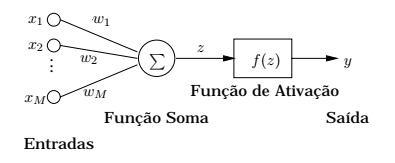
\includegraphics[width = 0.8\textwidth]{Caps/Figs/ref-teorico/mccul.png}
   \label{fig:neuronioartificial}
    \fonte{\cite{magalhaes2004redes}}
\end{figure}

Por exemplo, para o modelo de neurônio proposto por McCulloch-Pitts, a função de ativação é uma função degrau da seguinte forma~\cite{magalhaes2004redes}:
\begin{equation}
    f(z) = \left\{\begin{matrix}
    1, & \mbox{se } z > a, \\ 
    0, & \mbox{se } z \leq a.
    \end{matrix}\right.
\end{equation}

Arquiteturas neurais são tipicamente organizadas em camadas (Figura~\ref{fig:redeneuralCamadas}), com unidades que podem estar conectadas às unidades da camada posterior. A camada de entrada é onde os padrões são apresentados a rede. As camadas intermediárias é onde é feita a maior parte do processamento, através das conexões ponderadas, podendo ser consideradas como extratoras de características. Por último, a camada de saída é onde o resultado final é concluído e apresentado~\cite{andreCarvalhoRNA}.

\begin{figure}[!hbtp]
  \centering
   \caption{Camadas de uma rede neural.}
    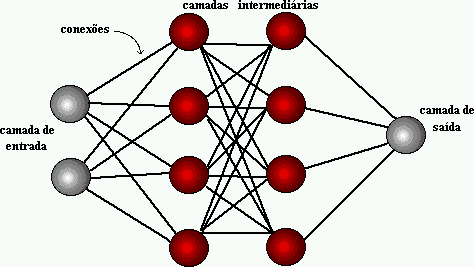
\includegraphics[width = 0.8\textwidth]{Caps/Figs/ref-teorico/rede-neural-camadas.jpg}
   \label{fig:redeneuralCamadas}
    \fonte{\cite{andreCarvalhoRNA}}
\end{figure}

A maioria dos modelos de redes neurais possui alguma regra de treinamento, onde os pesos de suas conexões são ajustados de acordo com os padrões apresentados. Em outras palavras, elas aprendem através de exemplos~\cite{andreCarvalhoRNA}. Isso é feito através de um processo iterativo de ajustes aplicado a seus pesos e o aprendizado ocorre quando a rede neural atinge uma solução generalizada para uma classe de problemas.


\subsection{Redes Neurais Convolucionais}
\label{sec:redesneuraisConvolucionais}
\nomenclature{CNN}{\textit{Convolutional Neural Network}}

Para a detecção de objetos prefere-se o uso de redes neurais convolucionais, do inglês \textit{Convolutional Neural Network} (CNN). Esta é uma variação das redes de múltiplas camadas, tendo sido inspirada no processo biológico de processamentos de dados visuais. Este tipo de rede vem sendo amplamente utilizada, principalmente nas aplicações de classificação, detecção e reconhecimento em imagens e vídeos~\cite{vargas2016estudo}.

Uma CNN é composta por diversas camadas (Figura~\ref{fig:CNN}) que utilizam a operação de convolução para realizar tal extração de características. Esta operação é realizada a partir de uma janela de dados deslizante, chamada de filtro convolutivo, que percorre toda a entrada da rede. O modelo pode conter diversos filtros, cujos valores são ajustados durante o processo de treinamento para a obtenção de características distintas a partir da entrada. Ao final, estas características extraídas se tornam entradas de um algoritmo de aprendizado aplicado a classificação ou regressão, de acordo com o tipo de problema. Ao final das camadas convolutivas, geralmente é utilizada uma sequência de camadas de neurônios conectados a todas as ativações das camadas anteriores, de forma análoga as camadas das ANNs (Seção~\ref{sec:redesneuraisArtificiais}). Estes modelos convolutivos tem obtidos ótimos resultados na visão computacional~\cite{oliveira2017redes}.

\begin{figure}[!hbtp]
  \centering
   \caption{Rede neural convolucional.}
    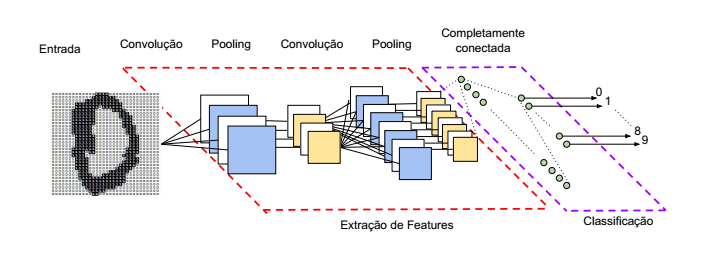
\includegraphics[width = 0.8\textwidth]{Caps/Figs/ref-teorico/CNN.png}
   \label{fig:CNN}
    \fonte{\cite{vargas2016estudo}}
\end{figure}

%\subsection{Processo de Treinamento}
%\label{subsec:treinamento}

%================================================================================]
%\section{Controle}
%\label{sec:controle}